\documentclass{article}
\usepackage{graphicx}
\usepackage{float}
\usepackage{amsmath}
\graphicspath{{images/}}
\usepackage{caption}
\captionsetup[figure]{position = below,}
\usepackage{listings}
\usepackage{xcolor}
\usepackage{amssymb}
 \usepackage{amsthm}
 \usepackage{amsfonts}
\usepackage{braket}
\DeclareCaptionFont{white}{\color{white}}
\DeclareCaptionFormat{listing}{%
\parbox{\textwidth}{\colorbox{gray}{\parbox{\textwidth}{#1#2#3}}\vskip-4pt}}
\captionsetup[lstlisting]{format=listing,labelfont=white,textfont=white}
\lstset{frame=lrb,xleftmargin=\fboxsep,xrightmargin=-\fboxsep, columns=fullflexible}


\title{\textbf{Analysis of \textit{Chaos Game} simulations with Pygame}}

\author{Indranil Ghosh\\Jadavpur University, PG I, Physics Department\\Email: indranilg49@gmail.com}

\date{\today}

\begin{document}
\maketitle

\tableofcontents

\begin{abstract}
This project is based on the dynamic simulations of various Chaos Game algorithms to produce fractal patterns, with the help of Pygame. Patterns to be discussed are Sierpinski’s Triangle, Barnsley’s fern and few restricted chaos game fractals. The Chaos game makes use of a random process to produce visualizations of self-similar fractal patterns on a plane. In this project some of the few fractal patterns, each with a description , its own chaos game rule and Pygame codes, to simulate its development are listed. Now, Pygame is a cross-platform set of python modules to create interactive video-games. These Pygame simulators make the visualizations of the pattern-generation grow with time, and very beautiful to look at. I also discuss some of the norms to be followed while using Pygame and its applications in scientific programming. 
\end{abstract}

\section{Introduction}
The algorithm of \textit{Chaos Game} was first developed by the british mathematician, \textbf{Michael Barnsley} around the year 1988, which produced some interesting fractal patterns. Generally, it refers to the method of generating the fixed point (attractor) of an iterated function system(IFS). Using the algorithm, the pattern is produced by iteratively creating a sequence of points, starting with an initial random point anywhere on the drawing platform. In the sequence, each point is the fraction of the distance between the previous point and a randomly chosen vertex (by rolling a dice, if human or by using a pseudo-random generator, if a computer!) of the n-gon.\\

\begin{itemize}
\item Although the algorithm is quite simple, the patterns formed, after continuous iterations, always exhibit infinite complexity and self similarity. Zooming a particular section of the fractal, results in the same pattern but with less density of points.\\
\item When the simulations are carried out, the fractal patterns grow and become clearer with time, with each iterations. If the n-gon is regular, the pattern formed is symmetric.
\end{itemize}

\section{Sierpinski's Triangle}
For constructing the Sierpinski's gasket, we consider 3 random vertices of a triangle and a random starting point. The distance factor \textbf{r} is $\frac{1}{2}$ (Distance factor is the fraction of the distance between a point plotted at a previous step and a randomly selected vertex of the triangle). This triangle is one of the most famous examples of self similar sets which can be recursively subdivided into smaller equally shaped trangles. It is named after the Polish mathematician \textbf{\textit{Waclaw Sierpinski}}.\\ \par

Let us consider an example. Let \textbf{A}, \textbf{B} and \textbf{C} be the three random vertices of a triangle and \textbf{St} be the starting point, also chosen randomly on the drawing platform. Generally, if we play manually by rolling a dice, we come up with a random integer in the range [1, 6] with an equal probability of $\frac{1}{6}$. We design the game in such a way that if we come up with a face 1 or 2, we move towards point A from the previous point and plot the new point halfway between. Similarly, if we come up with 3, 4 or 5, 6 we move halfway between B or C respectively. This process if continued for alarge number of iterations results in the formation of the Figure 1.

\begin{figure}[H]
\centering 
\noindent\makebox[\textwidth]{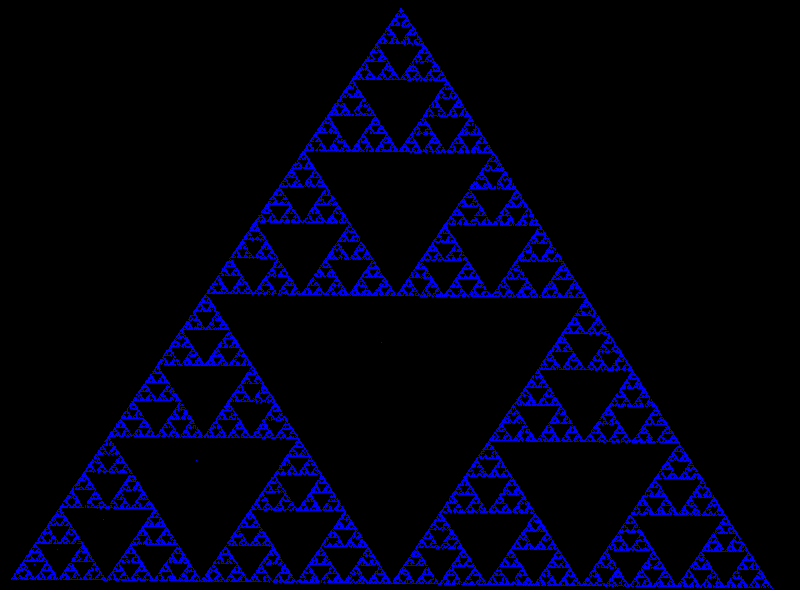
\includegraphics[scale=0.3]{sier}}%
\caption{Sierpinski's Triangle}
\end{figure}

Surely, the above algorithm is tremendously time and energy consuming for a human being to carry out for a large number of iteraions. So, Pygame! To simulate a dice roll, we take the help of a pseudo random number generator that generates a random number in the range [1, 6]. In the simulation, at first we choose 4 random points by clicking on arbitrary positions on the drawing surface. Nothing happens until we choose the $4^{th}$ point. As soon as it is chosen, the fractal pattern starts to grow. We do not set any upper bound in the while loop for the process to continue until we terminate it manually. Listed below is the software:
\begin{lstlisting}[language=Python, frame=single]
import random, pygame, sys
from pygame.locals import*
#set up the window
DISPLAYSURF=pygame.display.set_mode((800, 800))
#set up the colors
BLACK=(0, 0, 0)
BLUE=(0, 0, 255)
i=0
while True:
    for event in pygame.event.get():
        if event.type==QUIT:
            pygame.image.save(DISPLAYSURF, "Sierpinski.png")
            pygame.quit()
            sys.exit()
        elif event.type==MOUSEBUTTONUP:
            i+=1
            if i==1:
                A=(event.pos[0], event.pos[1])
                pygame.draw.circle(DISPLAYSURF,BLUE,A,0,0)
            elif i==2:
                B=(event.pos[0], event.pos[1])
                pygame.draw.circle(DISPLAYSURF,BLUE,B,0,0)
            elif i==3:
                C=(event.pos[0], event.pos[1])
                pygame.draw.circle(DISPLAYSURF,BLUE,C,0,0)
            elif i==4:
                St=(event.pos[0], event.pos[1])
                pygame.draw.circle(DISPLAYSURF,BLUE,St,0,0)
            else:
                pygame.quit()
                sys.exit()
    if i==4:
        x=random.randint(1, 6)
        if x in [1, 2]: St=((St[0]+A[0])//2, (St[1]+A[1])//2)
        elif x in [3, 4]: St=((St[0]+B[0])//2, (St[1]+B[1])//2)
        else: St=((St[0]+C[0])//2, (St[1]+C[1])//2)
        pygame.draw.circle(DISPLAYSURF, BLUE, St, 0, 0)
    pygame.display.update()
\end{lstlisting}

N.J.A Sloane's Online Encyclopedia of Integer Sequences also mentions this pattern as a triangle of integer sequence, read by rows, formed by reading Pascal's Triangle Mod 2. See A047999 and A001317.

\section{Pentagon Structures}
\subsection{n=5, r=$\frac{3}{8}$}
\begin{figure}[H]
\centering 
\noindent\makebox[\textwidth]{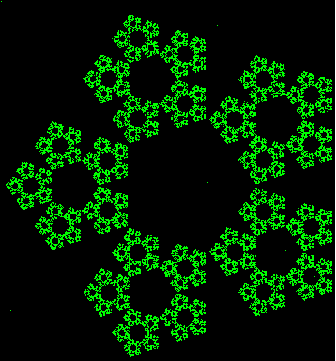
\includegraphics[scale=0.4]{pentagon1}}%
\caption{Pentagon 1}
\end{figure}

To construct the above fractal pattern, we need to follow almost the same algorithm as of Sierpinski's triangle, with slight alterations. The code is given below:
\begin{lstlisting}[language=Python, frame=single]
A=(217, 25)
B=(553, 134)
C=(553, 486)
D=(217, 595)
E=(10, 310)
St=(1, 1)

GREEN=(0, 255, 0)

pygame.draw.circle(DISPLAYSURF, GREEN, A, 0, 0)
pygame.draw.circle(DISPLAYSURF, GREEN, B, 0, 0)
pygame.draw.circle(DISPLAYSURF, GREEN, C, 0, 0)
pygame.draw.circle(DISPLAYSURF, GREEN, D, 0, 0)
pygame.draw.circle(DISPLAYSURF, GREEN, E, 0, 0)
pygame.draw.circle(DISPLAYSURF, GREEN, St, 0, 0)
#run the loop

while True:
    x=random.randint(1, 5)
    if x==1 : St=((St[0] + A[0])*3//8, (St[1] + A[1])*3//8)
    elif x==2 : St=((St[0] + B[0])*3//8, (St[1] + B[1])*3//8)
    elif x==3 : St=((St[0] + C[0])*3//8, (St[1] + C[1])*3//8)
    elif x==4 : St=((St[0] + D[0])*3//8, (St[1] + D[1])*3//8)
    else: St=((St[0] + E[0])*3//8, (St[1] + E[1])*3//8)
    pygame.draw.circle(DISPLAYSURF, GREEN, St, 0, 0)
    
    for event in pygame.event.get():
        if event.type==QUIT:
            pygame.image.save(DISPLAYSURF, "pentagon1.png")
    
            pygame.quit()
            sys.exit()

    pygame.display.update()
\end{lstlisting}
\subsection{n=5, r=$\frac{1}{2}$, restricted}
\begin{figure}[H]
\centering 
\noindent\makebox[\textwidth]{\includegraphics[scale=0.4]{penta}}%
\caption{Pentagon 2}
\end{figure}

The fractal pattern we see above is an example of a "restricted chaos game". Like the first pattern in this section, this pattern uses 5 vertices too, of a regular pentagon along with a random starting point, but with a distance factor $\frac{1}{2}$. This pattern has a keyword: restriction, because, to plot this, although we allow a point to be plotted midway towards a random vertex, the currently chosen vertex must be different than the previous one. The software is listed below:
\begin{lstlisting}[language=Python, frame=single]
A=(217, 25)
B=(553, 134)
C=(553, 486)
D=(217, 595)
E=(10, 310)
St=(1, 1)

RED=(255, 0, 0)

pygame.draw.circle(DISPLAYSURF, RED, A, 0, 0)
pygame.draw.circle(DISPLAYSURF, RED, B, 0, 0)
pygame.draw.circle(DISPLAYSURF, RED, C, 0, 0)
pygame.draw.circle(DISPLAYSURF, RED, D, 0, 0)
pygame.draw.circle(DISPLAYSURF, RED, E, 0, 0)
pygame.draw.circle(DISPLAYSURF, RED, St, 0, 0)
prev=random.randint(1, 5)

#run the loop
while True:
    l=[1, 2, 3, 4, 5]
    l.remove(prev)
    x=random.choice(l)
    if x==1:St=((St[0] + A[0])//2, (St[1] + A[1])//2)
    elif x==2:St=((St[0] + B[0])//2, (St[1] + B[1])//2)
    elif x==3:St=((St[0] + C[0])//2, (St[1] + C[1])//2)
    elif x==4:St=((St[0] + D[0])//2, (St[1] + D[1])//2)
    else:St=((St[0] + E[0])//2, (St[1] + E[1])//2)
    prev=x
    pygame.draw.circle(DISPLAYSURF, RED, St, 0, 0)

    for event in pygame.event.get():
        if event.type==QUIT:
            pygame.image.save(DISPLAYSURF, "pentagon2.png")
            pygame.quit()
            sys.exit()

    pygame.display.update()
\end{lstlisting}
\section{Square Structures [n=4, r=$\frac{1}{2}$, restricted]}
In this case, we always consider the number of vertices n=4 and the distance factor r=$\frac{1}{2}$. Without any restrictions, we get a random distribution of points all over the drawing platform, without any generation of interesting fractal pattern. So, we introduce various restrictions to observe some captivating fractal images.
\subsection{Type I}
\begin{figure}[H]
\centering 
\noindent\makebox[\textwidth]{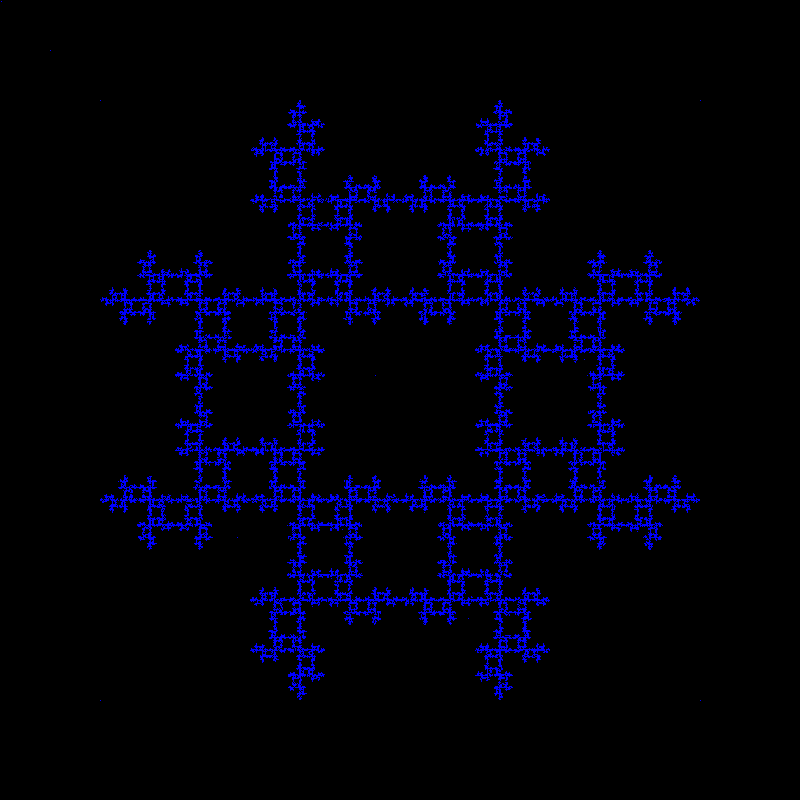
\includegraphics[scale=0.3]{square1}}%
\caption{Square 1}
\end{figure}
\begin{lstlisting}[language=Python, frame=single]
A=(100, 100)
B=(700, 100)
C=(700, 700)
D=(100, 700)
St=(1, 1)

BLUE=(0, 0, 255)

pygame.draw.circle(DISPLAYSURF, BLUE, A, 0, 0)
pygame.draw.circle(DISPLAYSURF, BLUE, B, 0, 0)
pygame.draw.circle(DISPLAYSURF, BLUE, C, 0, 0)
pygame.draw.circle(DISPLAYSURF, BLUE, D, 0, 0)
pygame.draw.circle(DISPLAYSURF, BLUE, St, 0, 0)
prev=random.randint(1, 4)

#run the loop
while True:
    l=[1, 2, 3, 4]
    l.remove(prev)
    x=random.choice(l)
    if x==1:St=((St[0] + A[0])//2, (St[1] + A[1])//2)
    elif x==2:St=((St[0] + B[0])//2, (St[1] + B[1])//2)
    elif x==3:St=((St[0] + C[0])//2, (St[1] + C[1])//2)
    else:St=((St[0] + D[0])//2, (St[1] + D[1])//2)
    prev=x
    
    pygame.draw.circle(DISPLAYSURF, BLUE, St, 0, 0)
    for event in pygame.event.get():
        if event.type==QUIT:
            pygame.image.save(DISPLAYSURF, "square1.png")
            pygame.quit()
            sys.exit()
            
    pygame.display.update()
\end{lstlisting}
\subsection{Type II}
\begin{figure}[H]
\centering 
\noindent\makebox[\textwidth]{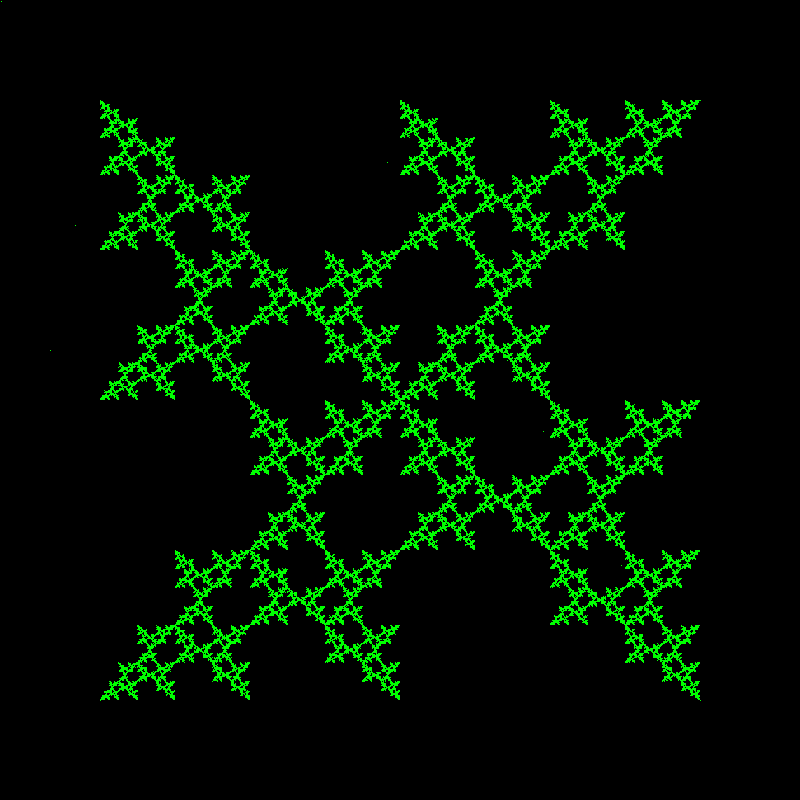
\includegraphics[scale=0.3]{square2}}%
\caption{Square 2}
\end{figure}

To construct the above figure, we plot 4 vertices of a regular square at first and a random starting point. Then in the simulation, we randomly chose a vertex in each iteration and plot a new point midway between the previously chosen point and the current vertex, but with the restriction that the current vertex should not be 1 place away in the anti-clockwise direction from the previously chosen vertex. In the code, we choose the same vertices and starting point as that of type I. Listed below is the code:
\begin{lstlisting}[language=Python, frame=single]
A=(100, 100)
B=(700, 100)
C=(700, 700)
D=(100, 700)
St=(1, 1)

GREEN=(0, 255, 0)

pygame.draw.circle(DISPLAYSURF, GREEN, A, 0, 0)
pygame.draw.circle(DISPLAYSURF, GREEN, B, 0, 0)
pygame.draw.circle(DISPLAYSURF, GREEN, C, 0, 0)
pygame.draw.circle(DISPLAYSURF, GREEN, D, 0, 0)
pygame.draw.circle(DISPLAYSURF, GREEN, St, 0, 0)
prev=random.randint(1, 4)

while True:
    l=[1, 2, 3, 4]
    l.remove(prev)
    x=random.choice(l)
    if x==1:
        St=((St[0] + A[0])//2, (St[1] + A[1])//2)
        prev=4
    elif x==2:
        St=((St[0] + B[0])//2, (St[1] + B[1])//2)
        prev=1
    elif x==3:
        St=((St[0] + C[0])//2, (St[1] + C[1])//2)
        prev=2
    else:
        St=((St[0] + D[0])//2, (St[1] + D[1])//2)
        prev=3
    
    pygame.draw.circle(DISPLAYSURF, GREEN, St, 0, 0)
    
    for event in pygame.event.get():
        if event.type==QUIT:
            pygame.image.save(DISPLAYSURF, "square2.png")
            pygame.quit()
            sys.exit()
            
    pygame.display.update()
\end{lstlisting}
Note that, in the restriction, if instead of not allowing the vertex lying 1 place away in the anti-clockwise direction from the previously chosen vertex, we do not chose the vertex 1 place away in the clockwise direction, we get the same image as Figure 5.
\subsection{Type III}
\begin{figure}[H]
\centering 
\noindent\makebox[\textwidth]{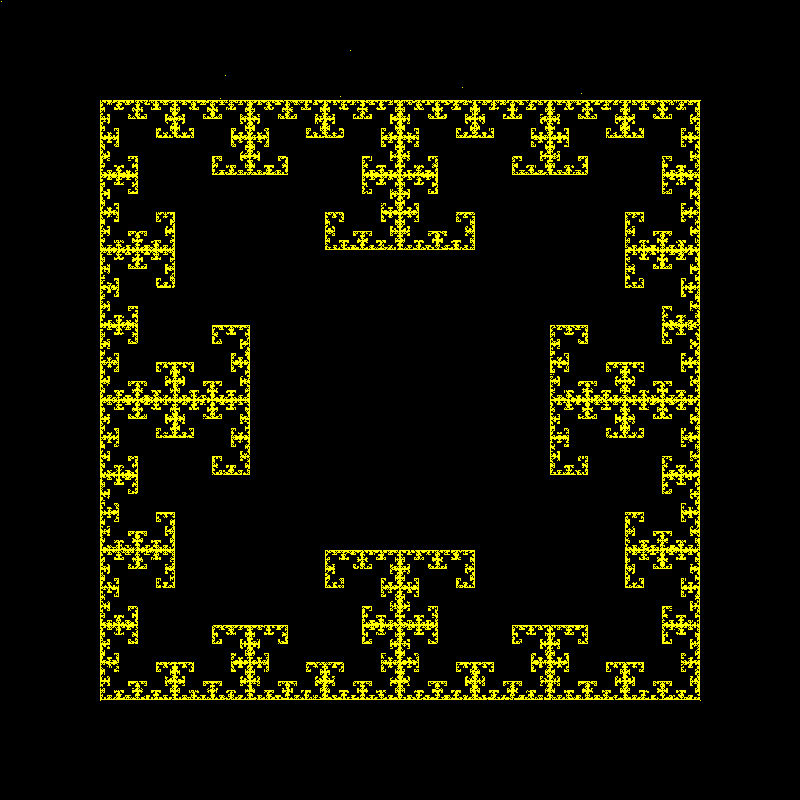
\includegraphics[scale=0.3]{square3}}%
\caption{Square 3}
\end{figure}
To construct this above gure, we select 4 vertices of a regular rectangle and a random starting point as usual. Then with each iteration, we select a random vertex and plot a point midway between the previous point and the current chosen vertex, with the restriction that this vertex must not be 2 places away from the previously chosen vertex. The code is listed below:
\begin{lstlisting}[language=Python, frame=single]
A=(100, 100)
B=(700, 100)
C=(700, 700)
D=(100, 700)
St=(1, 1)

YELLOW=(255, 255, 0)

pygame.draw.circle(DISPLAYSURF, YELLOW, A, 0, 0)
pygame.draw.circle(DISPLAYSURF, YELLOW, B, 0, 0)
pygame.draw.circle(DISPLAYSURF, YELLOW, C, 0, 0)
pygame.draw.circle(DISPLAYSURF, YELLOW, D, 0, 0)
pygame.draw.circle(DISPLAYSURF, YELLOW, St, 0, 0)
prev=random.randint(1, 4)

while True:
    l=[1, 2, 3, 4]
    l.remove(prev)
    x=random.choice(l)
    if x==1:
        St=((St[0] + A[0])//2, (St[1] + A[1])//2)
        prev=3
    elif x==2:
        St=((St[0] + B[0])//2, (St[1] + B[1])//2)
        prev=4
    elif x==3:
        St=((St[0] + C[0])//2, (St[1] + C[1])//2)
        prev=1
    else:
        St=((St[0] + D[0])//2, (St[1] + D[1])//2)
        prev=2
    pygame.draw.circle(DISPLAYSURF, YELLOW, St, 0, 0)

    for event in pygame.event.get():
        if event.type==QUIT:
            pygame.image.save(DISPLAYSURF, "square3.png")
            pygame.quit()
            sys.exit()
    
    pygame.display.update()
\end{lstlisting}
\section{Hexagon Structure, n=6, r=$\frac{1}{3}$}
\begin{figure}[H]
\centering 
\noindent\makebox[\textwidth]{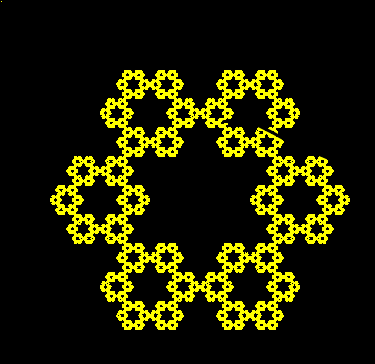
\includegraphics[scale=0.3]{hex}}%
\caption{Hexagon}
\end{figure}
Pygame code below:
\begin{lstlisting}[language=Python, frame=single]
A=(250, 140)
B=(100, 400)
C=(250, 660)
D=(550, 660)
E=(700, 400)
F=(550, 140)
St=(1, 1)

YELLOW=(255, 255, 0)

pygame.draw.circle(DISPLAYSURF, YELLOW, A, 0, 0)
pygame.draw.circle(DISPLAYSURF, YELLOW, B, 0, 0)
pygame.draw.circle(DISPLAYSURF, YELLOW, C, 0, 0)
pygame.draw.circle(DISPLAYSURF, YELLOW, D, 0, 0)
pygame.draw.circle(DISPLAYSURF, YELLOW, E, 0, 0)
pygame.draw.circle(DISPLAYSURF, YELLOW, F, 0, 0)
pygame.draw.circle(DISPLAYSURF, YELLOW, St, 0, 0)
#run the loop
while True:
    x=random.randint(1, 6)
    if x==1: St=((St[0] + A[0])//3, (St[1] + A[1])//3)
    elif x==2: St=((St[0] + B[0])//3, (St[1] + B[1])//3)
    elif x==3: St=((St[0] + C[0])//3, (St[1] + C[1])//3)
    elif x==4: St=((St[0] + D[0])//3, (St[1] + D[1])//3)
    elif x==5: St=((St[0] + E[0])//3, (St[1] + E[1])//3)
    else: St=((St[0] + F[0])//3, (St[1] + F[1])//3)
    pygame.draw.circle(DISPLAYSURF, YELLOW, St, 0, 0)

    for event in pygame.event.get():
        if event.type==QUIT:
            pygame.image.save(DISPLAYSURF, "hex.png")
            pygame.quit()
            sys.exit()

    pygame.display.update()
\end{lstlisting}
\section{Barnsley's Fern}
Like Sierpinski's gasket, this fern is another one of the basic fractal patterns, and named after the same person, Michael Barnsley we talked about earlier. The computer code that creates this pattern is also an example of IFS (iterated function system), like the ones we have beeen talking throughout. The Barnsley's fern shows, how one can built graphically beautiful structues from iterative use of mathematical formulas. The fern code developed by Barnsley also follows from the \textit{collage theorem}. Barnsley's fern uses four affine transformations, each of which looks like this:
\begin{gather}
f(x, y)=\begin{bmatrix}a & b \\ c & d \end{bmatrix}\begin{bmatrix}x\\y\end{bmatrix}+\begin{bmatrix}c\\d\end{bmatrix}
\end{gather}
Here \textbf{a} to \textbf{f} are the coefficients used in the affine transformations. We show three types of fractal leaves, their respective structues, affine transformations and Pygame programs to simulate their growth.

\subsection{Type \textit{Black Spleenwort}}
\begin{figure}[H]
\centering 
\noindent\makebox[\textwidth]{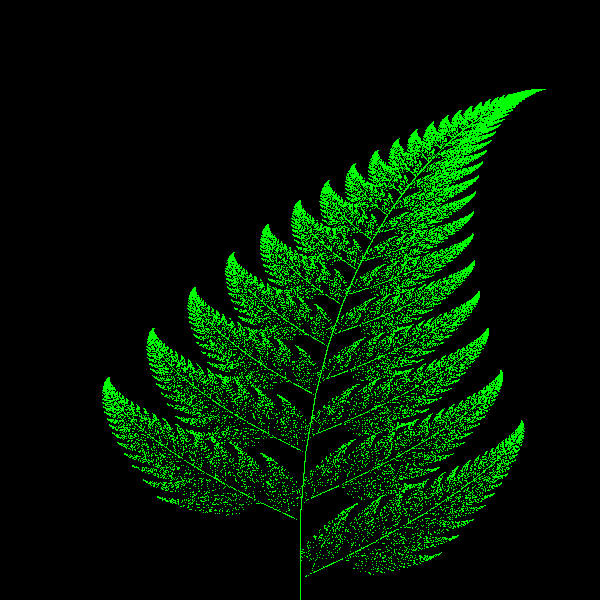
\includegraphics[scale=0.3]{BarnsleyFern}}%
\caption{Barnsley's Fern Type: \textit{Black Spleenwort}}
\end{figure}
To construct the fractal leaf, we require these transformations:
\begin{gather}
f_1(x, y)=\begin{bmatrix}0.00 & 0.00 \\ 0.00 & 0.16 \end{bmatrix}\begin{bmatrix}x\\y\end{bmatrix}
\end{gather}
\begin{gather}
f_2(x, y)=\begin{bmatrix}0.85 & 0.04 \\ -0.04 & 0.85 \end{bmatrix}\begin{bmatrix}x\\y\end{bmatrix} + \begin{bmatrix}0.00\\1.60\end{bmatrix}
\end{gather}
\begin{gather}
f_3(x, y)=\begin{bmatrix}0.20 & -0.26 \\ 0.23 & 0.22 \end{bmatrix}\begin{bmatrix}x\\y\end{bmatrix} + \begin{bmatrix}0.00\\1.60\end{bmatrix}
\end{gather}
\begin{gather}
f_4(x, y)=\begin{bmatrix}-0.15 & 0.28 \\ 0.26 & 0.24 \end{bmatrix}\begin{bmatrix}x\\y\end{bmatrix} + \begin{bmatrix}0.00\\0.44\end{bmatrix}
\end{gather}

\begin{itemize}
\item In simulating the growth, the first point is drawn at the origin ($X_0=0$, $Y_0=0$) and the successive points are iteratively plotted by randomly choosing one of the above four transformations.
\item $f_1$ transformation is chosen $1\%$ of the times and maps the base of the stem of the leaf, $f_2$ is chosen $85\%$ of the times and maps the smaller leaflets, $f_3$ and $f_4$ are each chosen $7\%$ of the times and maps the largest left-handed and the largest right-handed leaflet respectively.
\end{itemize}
Listed below is the Pygame code:
\begin{lstlisting}[language=Python, frame=single]
GREEN=(0, 255, 0)

X=[0.0]
Y=[0.0]
i=0

while True:
    r=random.random() 
    if r<=0.02:
        X+=[0.0, ]
        Y+=[0.16*Y[i], ]
    elif r<=0.86:
        X+=[0.85*X[i] + 0.04*Y[i], ]
        Y+=[-0.024*X[i] + 0.85*Y[i] + 1.6, ]
    elif r<=0.93:
        X+=[0.20*X[i] - 0.26*Y[i], ]
        Y+=[0.23*X[i] + 0.22*Y[i] + 1.6, ]
    else:
        X+=[-0.15*X[i] + 0.28*Y[i], ]
        Y+=[0.26*X[i] + 0.24*Y[i] + 0.44, ]

    pygame.draw.circle(DISPLAYSURF, GREEN, 
(int(X[i]*90 + 300), 600 - int(Y[i]*50)), 0, 0) 
    i+=1
\end{lstlisting}
\subsection{Type \textit{Thelypteridaceae}}

\begin{figure}[H]
\centering 
\noindent\makebox[\textwidth]{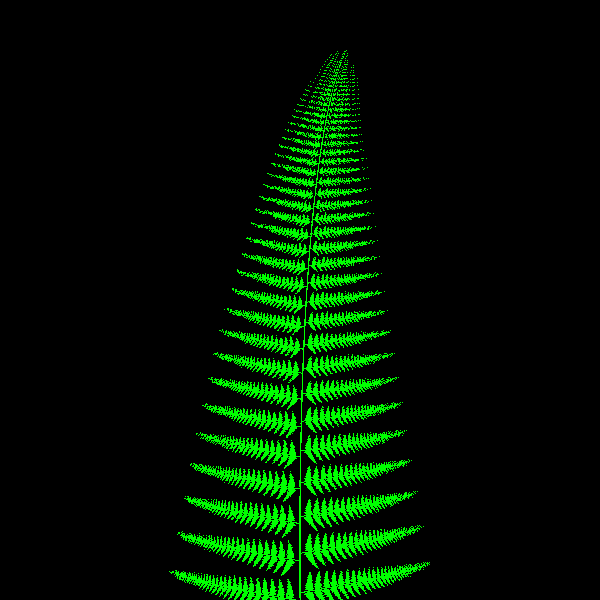
\includegraphics[scale=0.3]{BarnsleyFern2}}%
\caption{Barnsley's Fern Type: \textit{Thelypteridaceae}}
\end{figure}
To construct the fractal leaf, we require these transformations:
\begin{gather}
f_1(x, y)=\begin{bmatrix}0.00 & 0.00 \\ 0.00 & 0.25 \end{bmatrix}\begin{bmatrix}x\\y\end{bmatrix} + \begin{bmatrix}0.00\\-0.4\end{bmatrix}
\end{gather}
\begin{gather}
f_2(x, y)=\begin{bmatrix}0.95 & 0.005 \\ -0.005 & 0.93 \end{bmatrix}\begin{bmatrix}x\\y\end{bmatrix} + \begin{bmatrix}-0.003\\0.5\end{bmatrix}
\end{gather}
\begin{gather}
f_3(x, y)=\begin{bmatrix}0.035 & -0.2 \\ 0.16 & 0.04 \end{bmatrix}\begin{bmatrix}x\\y\end{bmatrix} + \begin{bmatrix}-0.09\\0.02\end{bmatrix}
\end{gather}
\begin{gather}
f_4(x, y)=\begin{bmatrix}-0.04 & 0.2\\ 0.16 & 0.04 \end{bmatrix}\begin{bmatrix}x\\y\end{bmatrix} + \begin{bmatrix}0.083\\0.12\end{bmatrix}
\end{gather}

\begin{itemize}
\item In simulating the growth, the first point is drawn at the origin ($X_0=0$, $Y_0=0$) and the successive points are iteratively plotted by randomly choosing one of the above four transformations.
\item $f_1$ transformation is chosen $2\%$ of the times, $f_2$ is chosen $84\%$ of the times, $f_3$ and $f_4$ are each chosen $7\%$ of the times.
\end{itemize}
Listed below is the Pygame code:
\begin{lstlisting}[language=Python, frame=single]
# GREEN=(0, 255, 0)

X=[0.0]
Y=[0.0]
i=0

while True:
    r=random.random() 
    if r<=0.02:
        X+=[0.0, ]
        Y+=[0.25*Y[i] - 0.4, ]
    elif r>0.02 and r<=0.86:
        X+=[0.95*X[i] + 0.005*Y[i] - 0.002, ]
        Y+=[-0.005*X[i] + 0.93*Y[i] + 0.5, ]
    elif r>0.86 and r<=0.93:
        X+=[0.035*X[i] - 0.2*Y[i] - 0.09, ]
        Y+=[0.16*X[i] + 0.04*Y[i] + 0.02, ]
    else:
        X+=[-0.04*X[i] + 0.2*Y[i] + 0.083, ]
        Y+=[0.16*X[i] + 0.04*Y[i] + 0.12, ]
    
    pygame.draw.circle(DISPLAYSURF, GREEN, (int(X[i]*90 + 300),
600 - int(Y[i]*80)), 0, 0)
    i+=1
    
    for event in pygame.event.get():
        if event.type==QUIT:
            pygame.image.save(DISPLAYSURF, "BarnsleyFern2.png")
            pygame.quit()
            sys.exit()

    pygame.display.update()
\end{lstlisting}
\subsection{Type \textit{Leptosporangiate}}

\begin{figure}[H]
\centering 
\noindent\makebox[\textwidth]{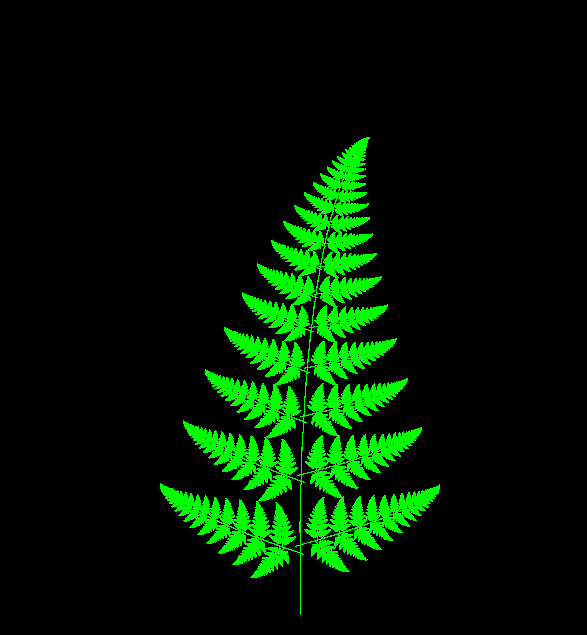
\includegraphics[scale=0.3]{BarnsleyFern3}}%
\caption{Barnsley's Fern Type: \textit{Thelypteridaceae}}
\end{figure}
To construct the fractal leaf, we require these transformations:
\begin{gather}
f_1(x, y)=\begin{bmatrix}0.00 & 0.00 \\ 0.00 & 0.25 \end{bmatrix}\begin{bmatrix}x\\y\end{bmatrix} + \begin{bmatrix}0.00\\-0.14\end{bmatrix}
\end{gather}
\begin{gather}
f_2(x, y)=\begin{bmatrix}0.85 & 0.02 \\ -0.02 & 0.83 \end{bmatrix}\begin{bmatrix}x\\y\end{bmatrix} + \begin{bmatrix}0.00\\1.0\end{bmatrix}
\end{gather}
\begin{gather}
f_3(x, y)=\begin{bmatrix}0.09 & -0.28 \\ 0.3 & 0.11 \end{bmatrix}\begin{bmatrix}x\\y\end{bmatrix} + \begin{bmatrix}0.00\\0.6\end{bmatrix}
\end{gather}
\begin{gather}
f_4(x, y)=\begin{bmatrix}-0.09 & 0.28\\ 0.3 & 0.09 \end{bmatrix}\begin{bmatrix}x\\y\end{bmatrix} + \begin{bmatrix}0.0\\0.7\end{bmatrix}
\end{gather}

\begin{itemize}
\item In simulating the growth, the first point is drawn at the origin ($X_0=0$, $Y_0=0$) and the successive points are iteratively plotted by randomly choosing one of the above four transformations.
\item $f_1$ transformation is chosen $2\%$ of the times, $f_2$ is chosen $84\%$ of the times, $f_3$ and $f_4$ are each chosen $7\%$ of the times.
\end{itemize}

Below is the Pygame code:
\begin{lstlisting}[language=Python, frame=single]
while True:
    r=random.random() 
    if r<=0.02:
        X+=[0.0, ]
        Y+=[0.25*Y[i] - 0.14, ]
    elif r>0.02 and r<=0.86:
        X+=[0.85*X[i] + 0.02*Y[i], ]
        Y+=[-0.02*X[i] + 0.83*Y[i] + 1.0, ]
    elif r>0.86 and r<=0.93:
        X+=[0.09*X[i] - 0.28*Y[i], ]
        Y+=[0.3*X[i] + 0.11*Y[i] + 0.6, ]
    else:
        X+=[-0.09*X[i] + 0.28*Y[i], ]
        Y+=[0.3*X[i] + 0.09*Y[i] + 0.7, ]
    
    pygame.draw.circle(DISPLAYSURF, GREEN, (int(X[i]*90 + 300),
600 - int(Y[i]*80)), 0, 0)
    i+=1
    
    for event in pygame.event.get():
        if event.type==QUIT:
            pygame.image.save(DISPLAYSURF, "BarnsleyFern3.png")
            pygame.quit()
            sys.exit()

    pygame.display.update()
\end{lstlisting}
\section{Conclusions}
\begin{itemize}
\item In our code, we need to keep in mind that the top left corner is coordinated (0, 0) in a pygame drawing surface and the value of Y-axis increases downwards.
\item Pygame does not allow floating point values. So, to get a convinient simulation, we need to map the pygame coordinates to a new coordinate system that suits our needs.
\item The dynamic simulations of fractals have turned out to be useful in scientific applications ranging from computer graphics, image compression, mathematical modeling, in video game industries, etc.
\end{itemize}
\section{Acknowledgement}
I would like to express my special thanks of gratitude to my Professors, Dr. Debasish Lohar and Dr. Subhankar Ray who helped me with golden suggestions. I am really thankful to them.

\begin{thebibliography}{10}
\bibitem{knuthwebsite}
\texttt{Rubin H. Landau, Manuel Jose Paez and Christian C. Bordeianu, \textit{"Computational Physics"}, New York: Wiley, 2007}
\bibitem{knuthwebsite}
\texttt{Al Sweigart, \textit{"Making Games with Python and Pygame"}, https://github.com/indrag49/Fractals-pygame}
\bibitem{knuthwebsite}
\texttt{Wolfram Mathworld, \textit{"Chaos Game"}, http://mathworld.wolfram.com/ChaosGame.html}
\bibitem{knuthwebsite}
\texttt{Wikipedia, \textit{"Barnsley's Fern"}, https://en.wikipedia.org/wiki/Barnsleyfern}
\bibitem{knuthwebsite}
\texttt{Indranil Ghosh, \textit{"Fractal-pygame"}, https://github.com/indrag49/Fractals-pygame}
\end{thebibliography}
\end{document}